\chapter{Privacidade}
\label{cap:privacidade}
% \chapter{Fundamentação teórica}
% \label{cap:fundamentacao}
% Mind Map para Fundamentação te: https://bit.ly/3P5rG3q

% Durante o estudo bibliográfico, foram lidos diversos artigos sobre a privacidade vs BC. O trabalho é organizar os artigos, criando um texto que convença o leitor de que eles são interligados e mostram cada ponto necessário para a resolução do problema, o objetivo e a justificativa vão ser incluídos posteriormente.

% Lembrar de mencionar que DLT e BC são intercambiáveis. Adicionar as siglas na seção de acronismos.

% Contextualização: Qual o papel da privacidade na sociedade moderna? Como atingir a privacidade em ambientes abertos e inseguros? Uma discussão sobre a influência da GDPR na Blockchain.

Privacidade e proteção de dados são duas questões inter-relacionadas de governança da Internet. A proteção de dados é um mecanismo legal que garante a privacidade. Geralmente definida como o direito de qualquer cidadão de controlar suas próprias informações pessoais e decidir sobre elas (divulgar informações ou não). É um direito humano fundamental, reconhecida na Declaração Universal dos Direitos Humanos, no Pacto Internacional sobre Direitos Civis e Políticos e em muitas outras convenções internacionais e regionais de direitos humanos \cite{DWObservatory2022:online}.

A diferença entre privacidade e proteção de dados, segundo Guamán \cite{dsguaman2016:online}, depende do país e das idiossincrasias da língua falada. Nos Estados Unidos da América (United States of America - USA), o termo privacidade domina as regras e práticas de processamento de dados pessoais, na União Européia (European Union - EU) o termo proteção de dados parece ser utilizado para se referir a mesma definição. Para evitar problemas de linguagem e suas diferenças, a EU utiliza o termo proteção de dados ao invés de privacidade para se referir a proteção do direito de privacidade no que diz respeito ao tratamento de dados pessoais.

Na segurança de dados os termos dados pessoais, informações pessoais ou Informações de Identificação Pessoal (Personally Identifiable Information - PII) são usados para descrever informações que podem ser usadas para identificar, contactar e localizar uma pessoa. Os termos privacidade, proteção de dados e PII são intercambiáveis nesta tese. %\cite{Personal37:online}.
% Esta tese preocupa-se com a privacidade e proteção dos dados pessoais, por isso os termos privacidade, proteção de dados e PII são intercambiáveis.

% No trabalho de Schwerin2018 menciona-se que PII e privacidade são termos intercambiáveis. Estou procurando uma forma de adicionar essa idéia na tese.

Segundo \citet{Schwerin2018}, a definição de PII muda com o desenvolvimento de tecnologias como blockchain, IA, Big Data e Internet das coisas (Internet of Things - IoT), pois aumentam a chance de reidentificar os dados. %apud 16.
Quase todos os dispositivos digitais usados por humanos e conectados à internet podem ser usados para rastrear sua origem. %(apud [17]).
Como esse tipo de dado está frequentemente ligado à identidade de um ser humano, ele deve ser protegido da mesma forma que outros direitos que esse indivíduo possui.

% O aumento da coleta de dados pelas organizações podem ferir o direito à privacidade do indivíduo, trazendo riscos e desafios a segurança \citep{Teixeira2019:article}. 

O direito à proteção do indivíduo pode estar em risco, devido ao aumento da coleta de dados pelas organizações, o que trás novos desafios à segurança \citep{Teixeira2019:article}. Em 2012 o conselho da união europeia começa a trabalhar na regulamentação EU 2016/679, entrando em vigor em 25 de maio de 2018, também chamada de GDPR (General Data Protection Regulation). Segundo \citet{gabriela_eu_2018:article} e \citet{Teixeira2019:article}, a nova lei revoga as diretrizes 95/46/EC, conhecida como a norma de proteção de dados da UE (EU Data Protection Directive). Com a intenção de dar mais controle aos cidadãos sobre seus dados pessoais, a GDPR impõe um conjunto de obrigações em respeito à guarda, processamento, coleta e divulgação de dados. A regulação é válida para qualquer organização que processe os dados e prevê multas pesadas quando a não conformidade com as regras são detectadas \citep{EuropeanCommission2016:misc}.

Nesse contexto, as empresas e governos fazem o papel de concentradores de dados, onde os usuários possuem um controle limitado sobre suas informações. As SNS (Social Network Sites) estão no foco principal, pois seus usuários disponibilizam uma grande quantidade de informações pessoais para esses sites. Para gerar modelos de negócios, essas organizações armazenam, distribuem, analisam informações confidenciais de PII de seus usuários \cite{Al-ZabenNasr2018:article}. Em abril de 2018, veio a público o caso da Cambridge Analytica, onde 50 milhões de perfis de usuários do Facebook foram violados. Apontado como o maior vazamento de dados pessoais até aquele momento; dados esses usados para criar ferramentas que direcionavam propagandas baseadas nos perfis coletados no Facebook, com o objetivo de influenciar as eleições americanas em 2015.

%e plataformas afins fazem a coleta de dados de PII \citep{Al-ZabenNasr2018:article}. Em busca de um ambiente mais aberto, a tecnologia BC ou DLT vem direcionar o direito de uso da PII para o usuário, assim como está definido na GDPR. Em contrapartida contra a centralização de dados, o BC é uma resposta.... 

%Para contrapor a grande concentração de dados de SNS --- temos tecnologias descentralizadas como o Blockchain. temos algumas respostas, como o Blockchain \citep{Schwerin2018}.

Para restaurar a confiança no mundo digital, uma solução proposta é a tecnologia Blockchain (abreviação BC) \citep{Schwerin2018}. Inicialmente a tecnologia foi desenvolvida para gerar imutabilidade, consenso e transparência em transações financeiras envolvendo a criptomoeda Bitcoin \citep{Nakamoto2009}. Ultimamente a tecnologia tem ganho atenção de pesquisadores que vão além das transações financeiras envolvendo criptoativos \citep{Al-ZabenNasr2018:article}. Também é conhecida como a tecnologia do livro-razão distribuído (Distributed Ledger Technology, DLT). E com ela, espera-se revolucionar a indústria, o comércio e mudar a economia em um escala global, garantindo a segurança em transações públicas e privadas \citep{Underwood2016:article}. % pois é imutável, transparente, criando confiança e segurança para transações públicas e privadas \citep{Underwood2016:article}.

Embora o BC seja uma saída a centralização de dados de SNS e afins, o mesmo não está livre de problemas. O BC é composto por bloco de dados imutáveis, que podem ser utilizados para rastrear a troca, guarda e distribuição de PII \citep{Al-ZabenNasr2018:article}. Com a legislação da GDPR, as organizações apenas podem processar os dados pessoais com o explicito consentimento do usuário. Mesmo depois de recebido o consentimento, os sujeitos tem o direito de atualizar seus dados, e o direito de revogar o consentimento a qualquer momento e também ter seus dados excluídos quando não houver mais razão para o processamento de seus dados ou se os mesmos foram capturados de maneira ilegal, ``direito ao esquecimento''. \citep{EuropeanCommission2016:misc} %retirado do artigo The Critical Success Factors of GDPR Implementation.

% Pesquisadores questionam a compatibilidade da GDPR com o BC, apontar uns 3 trabalhos. Apontam soluções.

% Podemos falar da privacidade na DLT.

% BC é uma tecnologia que chegou para ficar, dados escritos são imutáveis e a prova de fraudes. Mas é um risco ao PII/Privacidade do usuário, que pode ser utilizado de maneira "evil" (ver nos artigos, existe uma forma melhor de referir-se ao abuso de dados, normalmente praticado por empresas) por indivíduos ou empresas.

% Legislação Como a GDPR. Mesmo o blockchain pode ser usado para explorar os dados dos usuários, através de processos de mineração. Direito ao esquecimento Right to forget and should be erasable rights

%\textit{Rascunho:} Direito a privacidade na Blockchain. Como proteger os dados pessoais tem se tornado um tema cada vez mais importante \citep{Schwerin2018}. Uma preocupação crescente com o uso feito dos dados por grandes corporações. \cite{dsguaman2016:online} 
%[6]Privacy vs Data protection vs Information Security}. 
%Se o BC (Blockchain) precisa estar em compliance com a GDPR, pergunta: é possível? Se sim, o que precisa ser feito?


% OK. No ecossistema da BC \cite{Schwerin2018} menciona sobre a evolução e mudança de paradigma que irá influenciar cada fragmento do mundo que conhecemos, apud [10].

%Estratégias para proteger a privacidade. Segundo Hassan em seu artigo \cite{Hassan2020} a encriptação é uma das maneiras tradicionais de proteger a privacidade usada pela maioria dos sistemas para proteger os dados contra adversários e usuários não autorizados. Outra técnica é a anonimização de dados, que apud [23] \cite{Hassan2020} mostra que pode ser facilmente comprometidos. \cite{Dwork2006} propõe um trabalho que ao perturbar os dados, utilizando um processo de randomização, chamado Randomized Response proposto por S. L. Warner em 1965, a privacidade é alcançada através da negação plausível para qualquer entrada.

%Esse processo tem sido utilizado em sistemas onde não se conhece a capacidade de processamento do hardware.

% OK. Falar da GDPR. Contar um pouco da história. Verificar os artigos de referência se algum deles tem essa informação. Acho que o Schwerin2018 tem alguma informação relevante. Abaixo é uma explicação do site da UE.

% OK. A GDPR (General Data Protection Regulation) legisla como dados pessoais precisam ser coletados, processados e apagados. Entre os direitos que se destacam na lei, encontra-se o direito ao esquecimento \cite{Everythi34:online}.

%De acordo com Al-Zaben \cite{Al-ZabenNasr2018:article}, um número significativo de usuários fazem uso de redes sociais, fornecendo uma grande quantidade de PII para sites e aplicativos de redes sociais. Ainda afirma que o BC ganhou muita atenção de vários pesquisadores(incluir apuds? [7] [8]). Com a inclusão da GDPR os dados individuais precisam ser protegidos, ficando as instituições obrigadas a recolher o consentimento individual de cada usuário para coletar e compartilhar seus dados. Ainda é necessário a empresa garantir que seus dados possam ser removidos de sua base, conhecido como ``direito ao esquecimento"". Propõe-se a criação de um BC capaz de gerenciar PII utilizando organizações. Separando a persistência de PII de outros dados.

%Feng, no survey \cite{Feng2019} sobre proteção da privacidade no BC. Afirma que o BC é uma tecnologia disruptiva que funciona de maneira descentralizada. Sendo a tecnologia base para moedas digitais, como Bitcoin, operando de maneira distribuída sem o uso de uma entidade central.

% Parágrafo pode ir na seção de Blockchain - foco em IoT.
% Feng menciona o uso da tecnologia BC em IoT, por ser equipada com uma topologia descentralizada. O gerenciamento de equipamentos pode ser automatizado e a sincronização de dados pode ser fácil e rápida entre dispositivos IoT (Hud et al, 2017; Dorri et al. 2016; Conoscenti et al., 2016). Além disso o BC melhora a transparência e rastreabilidade de propriedade "Supply Chain Management Systems" (traduzir para o português) (várias referências). Além disso, a característica descentralizada do BC pode diminuir a pressão sobre servidores centralizados, para gerenciar infraestruturas de chaves públicas ou gerenciamento de sistemas de identidades (várias referências). Como contribuição apresenta uma análise crítica sobre mecanismos de defesa da privacidade no BC. 1) Definindo a privacidade além do usuário, incluindo a privacidade da transação. 2) Introduzindo ameaças existentes tanto para o usuário quanto para a transação no BC. 3) Introduzindo diversas tecnologias, especialmente técnicas de criptografia, que são usadas para proteger a privacidade no BC. 4) Os pontos para enteder a origem, objetivo e drawback de cada approach de proteção. 5) Avaliando o impacto de vários métodos para preservar a privacidade, em diversos protocolos em uso.

% Do ponto de vista de \cite{Schwerin2018} mostra que os especialistas que responderam aos seus questionamentos no seu estudo "delphi", que o BC não deve capturar dados pessoais de seus usuários. Feng apresenta mecanismos de privacidade, incluindo a criptografia. % Melhorar esse parágrafo, adicionar outros autores que apontam para soluções off-chain. Talvez a LGPD, tem um artigo do Teixeira, que menciona algo nesse sentido.

% Identificar trabalhos que apontam soluções para gravar dados "off-chain", apontar para as referências. O objetivo disso é mostrar o esforço que esses pesquisadores tem em relação a compliance com a LGPD e GDPR.

% Currently,  over  50  million  people  use  several   Social   Networking   Sites   (SNS)   and   have   made   available  a  vast  amount  of  PII  on  these  sites.  All  these  SNS  sites, other websites and mobile applications offer sign in or registration  for  premium  services.  PII  are  often  utilized  by  organizations  to  authenticate  a  customer’s  identity.  Since  most of these SNS sites and applications are for free, several studies found PII breaching by these organizations. Actually, these  organizations  store,  distribute,  analyse  sensitive  PII  information in order to generate business model through user profiling.  Tech  giants  uses  third  party  service  providing \cite{Al-ZabenNasr2018:article}

%\cite{article:BegumSNausheenF2018} Segurança dos Dados e Privacidade. Segundo Begum e Nausheen \cite{article:BegumSNausheenF2018}, segurança dos dados é comumente conhecida como confidencialidade, disponibilidade e integridade dos dados, garantindo que os dados não sejam usados por usuários não autorizados. Um plano de segurança de dados inclui apenas coletar as informações necessárias, mantê-las seguras e destruir qualquer informação que não seja mais necessária. Ainda, a privacidade dos dados é definida como o uso apropriado dos dados. Quando empresas e comerciantes usam dados ou informações que lhe são fornecidos, os dados devem ser usados de acordo com os fins acordados, sem divulgar as informações do consumidor. As abordagens para alcançar a privacidade são: encriptação, inclusão de ruídos e anonimização.

%\section{Um breve histórico da legislação antes da GDPR}
\section{Um breve histórico da GDPR}

Na Europa o desenvolvimento da GDPR foi uma jornada que percorre várias décadas, como o trabalho do \citet{Schwerin2018} demonstra. Com a transição da era da economia pós-industrial na década de 60, houve o surgimento de leis que procuravam estabelecer uma política para a proteção de dados. Em 1970, como resultado das mudanças governamentais e avanços na computação que permitiam recolher dados dos cidadãos, houve uma reflexão do paradigma da relação do estado com o individuo. Surgindo a primeira lei, que foi adotada pelo estado de Hesse na Alemanha em 1970, seguida da Suécia em 1973 e Alemanha, França, Dinamarca, Noruega e Áustria em 1978.

Na década de 80, começou a era da internalização dos dados, onde a Organização para Cooperação e Desenvolvimento (OCDE) formalizou a primeira iniciativa com guia para proteção, privacidade e fluxos transfronteiriços de dados pessoais para combater uma preocupação crescente sobre a ameaça da perda do controle das atividades de processamento.

A implementação nacional, entre 1982 e 1984, resultado do guia da OCDE para proteção de dados. Aqui em especial, o Reino Unido, com seu ato de 1984, e o ato Belga de proteção de dados em 1992, são vistos como marcos, criando uma estrutura abrangente em direção a proteção de dados. Ambos, acabaram sendo caracterizados como trabalhos apressados e forçaram a UE a uma ação de harmonização. Nessa época o desenvolvimento do PC, em conjunto com os avanços da Apple e da Microsoft, levaram a um crescimento exponencial do fluxo de dados, e também nessa época, se deu o desenvolvimento da internet como é conhecida hoje.

Harmonização europeia, entre 1995 e 2016, com a EU gerenciando a publicação da DPD (European Data Protection Directive) em 1996 na proteção e privacidade individuais em relação ao processamento de dados pessoais e o livre movimento desse tipo de dados. A diretiva serviu apenas como guia, sem o poder de lei, requisitando dos países participantes a necessidade de criar suas próprias leis locais. Como função a DPD tinha dois objetivos, garantir o direito a proteção de dados e a garantia do livre fluxo de dados pessoais entre os estados membros. A comissão da União Europeia fez uma proposta de reforma em 2012 para que a UE estabelecesse uma regulamentação de proteção abrangente. A regulação diferencia-se da diretiva, pois sobrescreve as leis nacionais, tornando as leis de aplicação imediata após ativação além de estabelecer mecanismos de execução.

Levou dois anos até que o parlamento europeu (PE) finalmente adotasse a GDPR proposta em 2014 e outros dois anos até finalizar a proposta e o plano de ação para sua implementação. Depois de meses de lóbi e a inclusão de mais de 3500 emendas a GDPR entrou em ação 20 dias depois de sua publicação no jornal oficial da UE. A GDPR foi planejada para entrar em vigor no dia 28 de maio de 2018. A intenção era que as organizações tivessem dois anos para se preparar e corrigir os processos de privacidade e políticas e se tornar compatível com as novas regras.

Os objetivos principais da GDPR eram dois, proteger os direitos, a privacidade e liberdade das pessoas naturais da UE e reduzir as barreiras para negócios facilitando o livre movimento de dados por toda UE. Sendo uma lei que influenciou os demais países a criarem seu próprio regulamento, inclusive o Brasil, com a Lei Geral de Proteção de Dados, conhecida como LGPD \citep{candido_historico_2021}. 

% aqui caberia colocar o trabalho da Patrícia PINHEIRO 2020 que pode falar mais da influência da GDPR no Brasil, sem ficar uma transição muito seca.

\section{LGPD - Lei Geral de Proteção de Dados}

%Preâmbulo:
As discussões sobre os problemas da privacidade podem ser resumidas por \citet{Nissenbaum+2009}, afirma que muitos artigos, livros e comentários chamam para uma reforma na lei ou na política, com o objetivo de criar defesas contra a corrosão da privacidade, devido ao aumento do uso sistemas tecnológicos. O argumento para proteger a privacidade significa restringir ou limitar o acesso as informações pessoais ou assegurar que as pessoas tenham controle sobre as próprias informações.

Apesar desse argumento, as pessoas se importam mais, não só com a simples restrição do fluxo de informação, mas assegurar que ele flua apropriadamente. Não se deve ter uma estrutura rígida, mas criar uma estrutura de integridade contextual que possa evoluir de acordo com a percepção de novas tecnologias e sistemas que possam ameaçar a privacidade; não apenas predizendo como as pessoas vão reagir aos sistemas, mas formulando uma maneira de aprimorar a avaliação desses sistemas e legitimar a resposta a eles \citep{Nissenbaum+2009}.

No Brasil, o direito à privacidade é um direito fundamental assegurado na Constituição Federal de 1988, no artigo 5o, inciso X, são invioláveis a intimidade, a vida privada, a honra e a imagem das pessoas, assegurado o direito a indenização pelo dano material ou moral decorrente de sua violação \citep{Constitucao1988:online}. No intuito de proteger os direitos fundamentais de liberdade e de privacidade, a LGPD estabelece o respeito à privacidade como um dos seus principais, no artigo 2o, inciso I, a disciplina da proteção de dados pessoais tem como fundamentos, o respeito a privacidade \citep{L13709_2018:online}.

Assim como na Europa a discussão sobre a efetividade e a observância da GDPR, também acontece no Brasil \citep{monteiro_efetividade_2019}. Segundo \citet{monteiro_efetividade_2019}, um dos grandes debates sobre a LGPD está ligado aos mecanismos de proteção de dados pessoais criados pela lei e a realização de seus objetivos. O objetivo da LGPD é proteger os direitos fundamentais da liberdade e de privacidade e o livre desenvolvimento da personalidade da pessoa natural. Para isso são analisados os mecanismos institucionais, preventivos e repressivos de proteção de dados pessoais previstos na LGPD.

Existem dois mecanismos de proteção de dados. O primeiro são as medidas de segurança que protegem e evitam problemas acidentais, ou acessos ilícitos, tratamento ou perda de dados pessoais. O segundo mecanismo são regras de boas práticas e de governança corporativa que estabelecem entre outras os padrões técnicos e procedimentos dos envolvidos no tratamento de dados pessoais \citep{monteiro_efetividade_2019}.

% falar de controladores, operadores e encarregados. pg 11 \cite{monteiro_efetividade_2019} ?

Ainda \citet{monteiro_efetividade_2019} fala sobre as boas práticas e de governança, ressaltando, que a LGPD faculta aos controladores e operadores de tratamentos de dados pessoais a formulação de suas próprias regras de governança, com base em seu artigo 50, logo abaixo:

%pode ser removido, se achar melhor. Coloquei aqui apenas como opção. E ter mais texto disponível.
\begin{quote}
``Art. 50. Os controladores e operadores, no âmbito de suas competências, pelo tratamento de dados pessoais, individualmente ou por meio de associações, poderão formular regras de boas práticas e de governança que estabeleçam as condições de organização, o regime de funcionamento, os procedimentos, incluindo reclamações e petições de titulares, as normas de segurança, os padrões técnicos, as obrigações específicas para os diversos envolvidos no tratamento, as ações educativas, os mecanismos internos de supervisão e de mitigação de riscos e outros aspectos relacionados ao tratamento de dados pessoais.''
\end{quote}

Recomenda-se que a implementação de um programa de governança em privacidade, com base nos princípios da segurança e prevenção, sendo essencial para que todos os requisitos necessários à proteção de dados pessoais sejam efetivados \citep{monteiro_efetividade_2019} e \cite{pinheiro_protecao_2020}.


Escrever sobre o livro da Patricia, que contem várias comparações interessantes com a GDPR. \cite{pinheiro_protecao_2020}

Falar da LGPD. \citep{carvalho_desafios_2019}, \citep{monteiro_efetividade_2019} e \citep{dadamos_fatores_2022}.

Além da Europa com a GDPR, outras iniciativas são importantes de serem mencionadas, como a legislação brasileira, Lei Geral de Proteção de Dados, que segundo... expande e aprimora a GDPR.

% Aqui abrimos para expandir cada um dos assuntos.
\chapter{Blockchain}

Inicialmente utilizada como livro razão de uma moeda digital online, descentralizada, ponto a ponto chamada Bitcoin, com o objetivo de manter a transparência e segurança nas transações realizadas entre os usuários, sem o uso de intermediários \cite{Nakamoto2009}. Sendo adaptada para além do processamento financeiro, como exemplo a rede Ethereum, que através da aplicação de uma máquina virtual, capaz de executar e armazenar códigos Turing-completo \cite{buterin_ethereum_2014}. A completude de Turing refere-se a capacidade de executar todos os comandos da máquina abstrata de Turing, sendo chamada de máquina universal. Com isso, a Blockchain passou de uma solução financeira para uma gama maior de aplicações.

% Blockchain é basicamente uma corrente de blocos que armazena todas as transações usando um livro razão público. A corrente cresce continuamente quando novos blocos são adicionados. O BLC pode trabalhar de maneira descentralizada só é possível através do uso de assinaturas digitais, \it{hash} criptográficas e algoritmos distribuídos de consenso. Todas as transações ocorrem de maneira descentralizada eliminando a necessidade de intermediários que validem as transações. Caraterísticas chave são descentralização, transparência, imutabilidade e auditabilidade. \cite{monrat2019survey}.

% Citar os papers que fazem referência as aplicações. Anotações do dia 14/08/2022.
% Os surveis do mendeley também podem ajudar a encontrar usos mais focados a ideia de privacidade.

% sistemas de transporte 

Entre as aplicações, destacam-se as criptomoedas, cadeia de abastecimento, serviços financeiros, gerenciamento de risco, internet das coisa. \cite{pinno2017controlchain}\cite{zheng2018blockchain}\cite{monrat2019survey}. 

\section{Arquitetura da Blockchain}
Vamos falar sobre esse assunto?

A DLT é formada por uma sequência de blocos, que mantém uma lista completa de todas as transações que foram efetuadas, assim como um livro razão público \cite{zheng2018blockchain}. A figura \ref{fig:blockchain-structure} ilustra um exemplo de estrutura da blockchain. Um bloco aponta para o anterior através de uma hash extraída do conteúdo desse bloco, também chamado de bloco pai. O primeiro bloco é chamado de bloco de geração (genesis block) e não possuí pai. E assim a cadeia de blocos é formada e recursivamente aponta para o bloco anterior, dessa forma é possível auditar a qualquer tempo se algum bloco do passado foi ou não modificado. 

% referência da figura: https://www.researchgate.net/figure/the-figure-of-Blockchain-structure_fig1_342208369
\begin{figure}[!htb]
\centering
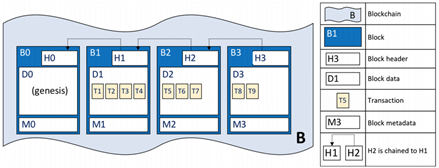
\includegraphics[width=12cm]{2-fundam/blockchain-structure.png}
\caption{Exemplo de estrutura da blockchain.}
\label{fig:blockchain-structure}
\end{figure}

% Inserir uma figura mostrando blocos ligados. \cite{zheng2018blockchain} pg 5 tem um bom exemplo.

A arquitetura tecnológica da blockchain é vista na figura \ref{fig:blockchain-architecture}, consistindo da camada de dados, rede, consenso, incentivo, contrato e aplicação. A camada de dados é constituída dos blocos de dados e carimbos de data/hora e guarda todos os dados de transações e informações em uma árvore merkle. A camada de rede inclui os protocolos P2P para comunicação, incluindo os mecanismos de propagação e verificação. A camada de consenso inclui os mecanismos de consenso, no qual permitem a cada um dos nós da rede a alcançar o consenso de maneira efetiva em um ambiente descentralizado e sem garantias de honestidade. %ambiente bizantino.
Para manter essa rede funcionando são oferecidos mecanismos de incentivo, integrando fatores econômicos na tecnologia blockchain, através de mecanismos de emissão e distribuição de incentivos econômicos. 
\cite{wu_application_2018}.

\begin{figure}[!htb]
\centering
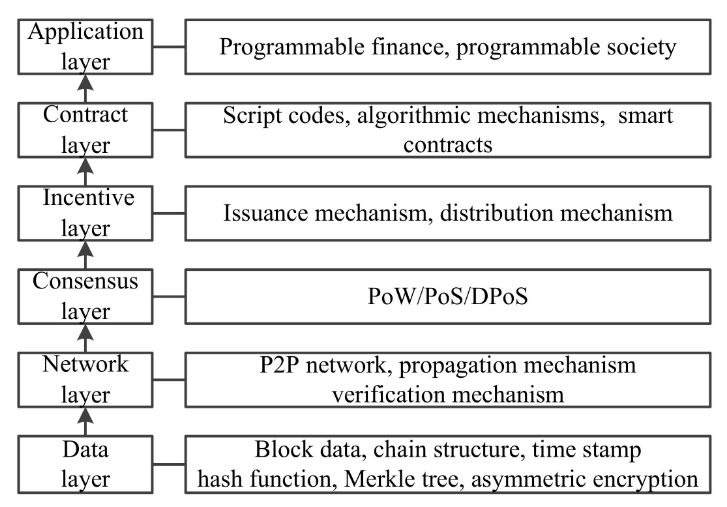
\includegraphics[width=12cm]{2-fundam/blockchain-architecture.png}
\caption{Exemplo de arquitetura da blockchain. \citep{wu_application_2018}}
\label{fig:blockchain-architecture}
\end{figure}

% \cite{monrat2019survey} chama de Taxonomia de sistemas blockchain, quando classifica os três tipos de blockchain, como público, privado e consórcio [45]. Já \citet{wu_application_2018} chamada de classificação da blockchain e os chamas de categoria, baseado no artigo [19]

\section{Aplicações}

% Interessante lembrar que o bitcoin não é a blockchain, mas a aplicação de maior sucesso da tecnologia \citep{monrat2019survey}.

Finanças, energia, gerenciamento de identidade, Sistemas de reputação, segurança e privacidade.

Na área da finanças \citet{zheng2018blockchain} mostra que tanto a Bitcoin \citep{Nakamoto2009} como \citet{linux_foundation_hyperledger_2015} trouxeram um grande impacto no modelo tradicional de negócios. Apontado como tecnologia capaz de promover a disruptura do mundo bancário. Podendo ser aplicada a muitas áreas, incluindo a compensação e liquidação de ativos financeiros. Mostrou que existem casos de negócios reais, como a garantia de derivativos financeiros, que podem alavancar o blockchain para reduzir custos e riscos. A tecnologia ainda despertou a atenção de grandes empresas de software, tanto a Microsoft Azure (falta referência) e IBM (falta referência) estão oferecendo serviços de Blockchain-as-a-Service.

Na área de energia, o maior uso da tecnologia está relacionado com micro-redes (microgrids). Uma micro-rede é uma solução localizada de um conjunto de fontes e cargas integradas e gerenciadas com o objetivo de aprimorar a produção de energia e eficiência. Os sistemas elétricos podem ser geradores distribuídos, de energia reutilizável, e componentes de armazenamento de energia criados e organizados por diferentes organizações ou provedores de energia. Uma das principais vantagens da tecnologia de micro-redes é que ela não apenas permite que moradores e outros consumidores de energia elétrica, como fábricas, tenham acesso à energia necessária, mas também podem produzir e vender o excesso de energia para a rede. Blockchain pode ser usado para facilitar, registrar e validar transações de compra e venda de energia em micro-redes \citep{monrat2019survey}.

No gerenciamento de identidade poderia substituir o tradicional documento de identidade, como carteira de motorista, carteira de identidade nacional e passaporte. Ao permitir uma abordagem decentralizada e criptografada, é possível fornecer um ambiente capaz de proteger a identidade do indivíduo contra roubo ou reduzir atividades fraudulentas. Ao permitir que um usuário crie uma identidade sem o uso de nome de usuário e senha, oferecendo recursos para o acesso às suas informações pessoais. Ao incluir a verificação de identidade com esse princípio da blockchain descentralizada, um ID digital pode ser gerado. Esse ID pode ser atribuído a todas as transações online semelhantes a uma marca d'água. Ajudando organizações a eliminar possíveis fraudes, permitindo a verificação de identidades em tempo real \citep{monrat2019survey}.

Sistemas de reputação são uma importante medida de como a comunidade confia no indivíduo. Quanto maior a reputação, mais confiável é a pessoa em relação a comunidade. A reputação pode ser avaliada por suas transações e interações com a comunidade. Evitando problemas de falsificação de registros, usados para enganar sistemas centralizados de reputação. Exemplo, no comércio eletrônico, muitos sites permitem que usuários inscritos gerem algum tipo de reputação em torno de produtos. Se um grupo de usuários falsos forem criados para artificialmente criar reputação de produtos, pode ferir a confiabilidade do comércio eletrônico responsável pelo sistema. Sendo que a DLT pode oferecer soluções para este problema. \citep{zheng2018blockchain}.




mostrou que existem casos de negócios reais, como a garantia de derivativos financeiros, que podem alavancar o blockchain para reduzir custos e riscos. Blockchain também chamou muita atenção aos olhos de grandes empresas de software

\chapter{Mecanismos de Privacidade}
Begum \cite{article:BegumSNausheenF2018}.

\chapter{Privacidade Diferencial}
\label{cap:privacidadediferencial}

\chapter{Privacidade no Blockchain}
\label{cap:blockchain}
Feng \cite{Feng2019}.

\section{Privacidade Diferencial no Blockchain}
Hassam \cite{Hassan2020}. % Deveria ser o survey.

% \chapter{Alguns exemplos}
% \label{cap:exemplos}
% 
% % figuras estão no subdiretório "figuras/" dentro deste capítulo
% \graphicspath{\currfiledir/figuras/}
% 
% %=====================================================
% 
% \section{Guias de \LaTeX}
% 
% Este modelo contém exemplos para os padrões de inserção de figuras, tabelas, listas de itens, bibliografia, etc. Em caso de dúvidas ou discordância, Pode-se entrar em contato com a direção ou secretaria do programa. Obviamente, críticas (construtivas) e sugestões são muito bem-vindas.
% 
% Para aprender a usar \LaTeX, um bom guia introdutório disponível na Internet é \cite{oetiker07}, que também tem uma versão em português. Para tópicos mais avançados consulte \cite{goossens93}.
% 
% %=====================================================
% 
% \section{Estrutura do texto}
% 
% Para melhorar a legibilidade do texto, deve ser evitado o uso de subdivisões mais profundas que a subseção (por exemplo, subsubseções). Se elas forem absolutamente necessárias, não devem ser numeradas. Deve-se analisar a possibilidade de uso de uma lista de itens em seu lugar. O número de níveis de texto do documento não deve exceder três: capítulo, seção e subseção. O uso de mais que três níveis dificulta a leitura e prejudica muito a estética do texto.
% 
% %=====================================================
% 
% \section{Estilo de redação}
% 
% Ao elaborar o texto da dissertação ou da tese, o mais indicado é o uso do verbo na forma impessoal. Exemplos:
% 
% \begin{itemize}
% \item ... utilizaram-se os seguintes dados ...
% \item ... elaborou-se de forma precisa ...
% \item ... trata-se os algoritmos ...
% \item ... foram obtidos resultados significativos ...
% \end{itemize}
% 
% Além disso, deve-se a todo custo evitar a ``linguagem de revista'', com expressões como ``sensacional'', ``impressionante'', ``monstruoso'', etc (por exemplo: ``Os resultados obtidos são sensacionais, sobretudo considerando a monstruosa margem de erro.'').
% 
% %=====================================================
% 
% \section{Alguns exemplos}
% 
% Esta seção traz algus exemplos de elementos típicos de um texto científico, como figuras, tabelas e fórmulas matemáticas.
% 
% %=====================================================
% 
% \subsection{Exemplo de figura}
% 
% A forma sugerida para incluir figuras em um documento \LaTeX\ é importá-las usando o pacote \texttt{graphicx}. Como formatos gráficos sugere-se:
% 
% \begin{itemize}
% 
% \item Formatos \emph{raster}, como PNG (\emph{Portable Network Graphics}) ou JPG (\emph{Joint Photographic Experts Group}) para fotografias; procure usar uma resolução de ao menos 150 dpi (\emph{dots per inch}).
% 
% \item Formatos vetoriais, como PDF (\emph{Portable Document Format}) ou EPS (\emph{Extended PostScript}) para diagramas e gráficos\footnote{NUNCA use JPG ou GIF para desenhos vetoriais, pois o resultado final geralmente fica borrado.}.
% 
% \end{itemize}
% 
% A maior parte das ferramentas permite exportar figuras nesses formatos (a figura do exemplo foi produzida com o \emph{Inkscape}, um programa livre multiplataforma). A figura \ref{fig:comun-intra-inter} mostra um exemplo de inclusão de figura em PDF.
% 
% % exemplo de inserção de figura
% \begin{figure}[!htb]
% \centering
% 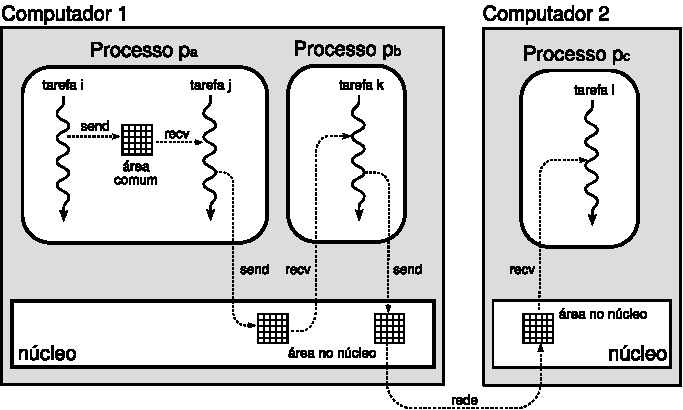
\includegraphics[width=12cm]{exemplo-figura.pdf}
% \caption{Comunicação inter-processos.}
% \label{fig:comun-intra-inter}
% \end{figure}
% 
% Para mais informações consulte \cite{goossens93}.
% 
% %=====================================================
% 
% \subsection{Exemplo de tabela}
% 
% Tabelas são elementos importantes de um documento. No \LaTeX\ as tabelas podem ser objetos flutuantes (definidas no ambiente \texttt{table} e referenciadas por números usando \texttt{label} e \texttt{ref}) ou objetos fixos simples, criados pelo ambiente \texttt{tabular}. A tabela \ref{tab:modelos} é um exemplo de tabela flutuante, cuja posição no texto pode variar em função das quebras de página.
% 
% \begin{table}[!htp]
% \centering
% \caption{Os 16 modelos centrais do UCON$_{\mathrm{ABC}}$}
% \label{tab:modelos}
% \begin{tabular}{|c|cccc|}
% \cline{2-5}
% \multicolumn{1}{c|}{}& 0 (imutável) & 1 (\emph{pre-update}) & 2 (\emph{on-update}) & 3 (\emph{pos-update}) \\
% \hline
% \texttt{preA} & \textbullet & \textbullet & -- & \textbullet \\
% \hline
% \texttt{onA} & \textbullet & \textbullet & \textbullet & \textbullet \\
% \hline
% \texttt{preB} & \textbullet & \textbullet & -- & \textbullet \\
% \hline
% \texttt{onB} & \textbullet & \textbullet & \textbullet & \textbullet \\
% \hline
% \texttt{preC} & \textbullet & -- & -- & -- \\
% \hline
% \texttt{onC} & \textbullet & -- & -- & -- \\
% \hline
% \end{tabular}
% \end{table}
% 
% %=====================================================
% 
% \subsection{Exemplo de fórmula}
% 
% Equações destacadas devem ser numeradas como mostra a equação \ref{eq:relatividade}:
% 
% \begin{equation}
% E = m \times c^2
% \label{eq:relatividade}
% \end{equation}
% 
% %=====================================================
% 
% \subsection{Exemplos de código-fonte}
% 
% Códigos-fonte podem ser produzidos de forma simples através do ambiente \texttt{verbatim}, como mostra este exemplo:
% 
% \begin{footnotesize}
% \begin{verbatim}
% #include <stdio.h>
% 
% int main (int argc, char *argv[])
% {
%    int i ;                           // uma variavel local
% 
%    for (i=0; i< 100; i++)            // um laço for
%       printf ("i vale %d\n", i) ;    // uma saída na tela
% }
% \end{verbatim}
% \end{footnotesize}
% 
% No entanto, é preferível usar pacotes especializados para a edição ou inclusão de códigos-fonte, como o pacote \texttt{listings}. Eis um exemplo de código-fonte escrito com esse pacote:
% 
% % exemplo de código-fonte definido no próprio texto
% 
% \begin{lstlisting}
% #include <stdio.h>
% 
% int main (int argc, char *argv[])
% {
%    int i ;                           // uma variável local
% 
%    for (i=0; i< 100; i++)            // um laço for
%       printf ("i vale %d\n", i) ;    // uma saída na tela
% }
% \end{lstlisting}
% 
% Esse pacote também permite incluir códigos-fonte de arquivos externos. Eis um exemplo:
% 
% % exemplo de código-fonte incluso
% 
% \lstinputlisting{2-fundam/exemplo.c}
% 
% %=====================================================
% 
% \subsection{Exemplo de algoritmo}
% 
% Os pacotes \texttt{algorithm} e \texttt{algorithmic} permitem formatar algoritmos facilmente. Eis um exemplo:
% 
% \begin{algorithm}[H]
% \caption{Ações de $s_i$ ao encerrar um ciclo:}
% \label{alg:on-period-ending}
% \begin{small}
% \begin{algorithmic}[1]
% \FORALL{$x \in \mathcal{K}_i$}
%   \STATE{$\mathit{banned}_i(x) \gets$ FALSE}
%   \STATE{$mi_i(x) \gets 0$}
%   \STATE{$mm_i(x) \gets 0$}
%   \STATE{$\mathit{age}_i(x) \gets \mathit{age}_i(x) + 1$}
%   \IF{$\mathit{age}_i(x) = \mathit{age}_\mathit{max}$}
%      \STATE{$\mathcal{K}_i \gets \mathcal{K}_i - \{x\}$}
%      \COMMENT{``esquece'' do servidor $x$}
%      \STATE{remove as informações locais sobre $x$}
%      \STATE{envia $\mathit{notify}(x,\mathit{undef})$ ao grupo de confiança $\mathcal{T}_i$}
%   \ENDIF
% \ENDFOR
% \end{algorithmic}
% \end{small}
% \end{algorithm}
%  
% %=====================================================
% 
% \subsection{Exemplo de citação}
% 
% Como afirmou Maquiavel em seu livro \emph{O Príncipe}:
% 
% \begin{quote}
% ``Nada é mais difícil de instituir, mais perigoso de conduzir, mais incerto no seu sucesso, do que liderar a introdução de uma nova ordem de coisas... O inovador faz inimigos em todos aqueles que prosperavam sobre as antigas regras, e somente tíbio suporte é esperado daqueles que prosperariam na novidade, porque os homens são geralmente incrédulos, nunca realmente confiam nas coisas novas, a menos que as tenham testado em experiência''.
% \end{quote}
% 
% %=====================================================
% 
% \section{Uma seção}
% 
% \subsection{Uma subseção}
% 
% \subsubsection{Uma subsubseção}
% 
% %=====================================================

% \section{Conclusão}
% 
% Todo capítulo (com exceção da introdução e da conclusão) deve encerrar com uma pequena conclusão local, resumindo os tópicos apresentados no capítulo e preparando o leitor para o próximo capítulo (exceto se esse for a conclusão geral). Caso o capítulo tenha apresentado resultados obtidos pelo próprio autor, estes devem ser sucintamente relembrados aqui.
% 
%=====================================================
